\documentclass[12pt]{article}\usepackage[english]{babel}
\usepackage[utf8]{inputenc}
\usepackage[T2A]{fontenc}
\usepackage{amssymb}
\usepackage{enumerate}
\usepackage{hyperref, fancyhdr, lastpage, fancyvrb, tcolorbox, titlesec}
\usepackage{array, tabularx, colortbl}
\usepackage{tikz}
\usepackage{venndiagram}
\usepackage{amsthm, bm}
\usepackage{relsize}
\usepackage{amsmath,physics}
\usepackage{mathtools}
\usepackage{subcaption}
\usepackage{scalerel}
\usepackage{theoremref}
\usepackage{circuitikz}
\usepackage{geometry}
\usepackage{stmaryrd}
\usepackage{forest}
\usepackage{cancel}
\usepackage{faktor}
\usepackage{gensymb}
\usepackage{fontawesome5}
\usetikzlibrary{automata, arrows, positioning, shapes}
\usetikzlibrary{decorations.pathmorphing}
\useforestlibrary{linguistics}
\usepackage{cleveref} % Must be loaded LAST

\ExplSyntaxOn
\NewDocumentCommand{\opair}{m}
 {
  \langle\mspace{2mu}
  \clist_set:Nn \l_tmpa_clist { #1 }
  \clist_use:Nn \l_tmpa_clist {,\mspace{3mu plus 1mu minus 1mu}\allowbreak}
  \mspace{2mu}\rangle
}
\ExplSyntaxOff

\hypersetup{
    colorlinks=true,
    linktoc=all,
    linkcolor=blue,
    citecolor=blue
}

% \setlength\parindent{0pt}

\newcommand{\N}{\mathbb{N}}
\newcommand{\Z}{\mathbb{Z}}
\newcommand{\Q}{\mathbb{Q}}
\newcommand{\R}{\mathbb{R}}
\newcommand{\E}{\mathbb{E}}
\newcommand{\M}{\mathbb{M}}
\newcommand{\bbH}{\mathbb{H}}
\newcommand{\bbP}{\mathbb{P}}

\newcommand{\vars}{\operatorname{Vars}}
\newcommand{\free}{\operatorname{Free}}

\newcommand{\logand}{\; \& \;}

\newcommand{\calA}{\mathcal{A}}
\newcommand{\calS}{\mathcal{S}}
\newcommand{\calD}{\mathcal{D}}
\newcommand{\calL}{\mathcal{L}}
\newcommand{\calZ}{\mathcal{Z}}
\newcommand{\calQ}{\mathcal{Q}}
\newcommand{\calR}{\mathcal{R}}
\newcommand{\calN}{\mathcal{N}}
\newcommand{\calM}{\mathcal{M}}
\newcommand{\calF}{\mathcal{F}}
\newcommand{\calI}{\mathcal{I}}
\newcommand{\calP}{\mathcal{P}}
\newcommand{\calC}{\mathcal{C}}
\newcommand{\calG}{\mathcal{G}}
\newcommand{\calB}{\mathcal{B}}
\newcommand{\calU}{\mathcal{U}}

\newcommand{\continuum}{\mathfrak{c}}
\newcommand{\ufnumber}{\mathfrak{u}}
\newcommand{\domnumber}{\mathfrak{d}}

\newcommand{\cof}{\operatorname{cof}}
\newcommand{\dom}{\operatorname{Dom}}
\newcommand{\rng}{\operatorname{Rng}}

\newcommand{\MA}{\mathsf{MA}}

\newcommand{\fa}{\kern.05em\ensuremath\forall\kern-.22em\rotatebox{69}{\rule{.73em}{.4pt}}}
\newcommand{\ex}{\kern.05em\ensuremath\exists\kern-.03em\rotatebox{90}{\rule{.68em}{.35pt}}}

\newcommand{\dequiv}{\stackrel{\text{деф.}}{\longleftrightarrow}}

\newcommand{\db}[1]{\llbracket #1 \rrbracket}

\DeclareMathOperator*{\bigand}{\scalerel*{\&}{\prod}}
\DeclareMathOperator*{\bigor}{\scalerel*{\lor}{\sum}}

\theoremstyle{definition}
\newtheorem*{definition}{Definition}
\newtheorem*{theorem}{Theorem}
\newtheorem{claim}{Claim}
\newtheorem{lemma}{Lemma}
\newtheorem*{fact}{Fact}
\theoremstyle{remark}
\newtheorem*{remark}{Remark}

\title{On `Ultrafilters with small generating sets`}
\author{Todor Dukov}

\begin{document}
\maketitle

\section*{Introduction}

The aim of this document is to give a better understanding of \cite{BlassShelah1989} by filling in details while also giving a high-level overview of the construction.
We will talk about the ultrafilter number $\ufnumber$ and the dominating number $\domnumber$.
The main result of \cite{BlassShelah1989} is the consistency of
\[
  \ufnumber = \kappa < \domnumber = \continuum = \lambda
\]
for any regular $\kappa, \lambda$, such that $\kappa < \lambda$.

The way we would do that is by first adding (with finite support iteration) $\lambda$-many Cohen reals and then very carefully adding $\kappa$-many Mathias reals.
We shall treat the construction of the ultrafilter for Mathias with utmost care, so that
\begin{enumerate}
  \item It does not ruin any work of the Cohen forcing for the dominating number.
  \item The same Mathias real would be added no matter what level we are on the Cohen forcing iteration.
\end{enumerate}
It is obvious why we have the first requirement.
After Cohen forcing we would have $\domnumber = \continuum = \lambda$ (if we start with a model of \textbf{CH}).
We would like to keep it that way during every step of the Mathias forcing.
It is not so obvious why we need to satisfy the second requirement.
If we satisfy the second requirement we would get what is called a matrix iteration.
This would allow for more precise control of the model because we can attack the problem from two sides instead of one which would also help with the first requirement.

Let me try to explain it better.
Let $V$ be the ground model.
Suppose the added Cohen reals are $\{ r_\alpha \}_{\alpha < \lambda}$ and the added Mathias reals are $\{ s_\beta \}_{\beta < \kappa}$.
For $\alpha < \lambda$ and $\beta < \kappa$ denote
\[
  V_{\alpha, \beta} = V[\{ r_\gamma \}_{\gamma < \alpha}][\{ s_\delta \}_{\delta < \beta}].
\]
What we would like is for $V_{\alpha + 1, \beta + 1}$ to be related to both $V_{\alpha, \beta + 1}$ and $V_{\alpha + 1, \beta}$.
Being related to both would guarantee the niceties of both our Mathias forcing and Cohen forcing.
This is how it looks visually:
\begin{figure}[htbp]
\noindent\hspace*{-1.5cm}
\scalebox{0.68}{%
\begin{tikzpicture}[
    scale=1.2,
    >=Stealth,
    dot/.style={circle, fill=black, inner sep=1.2pt},
    bigdot/.style={circle, fill=black, inner sep=2pt}
]

    % --- Corners / Outer Bounds ---
    \coordinate (V00) at (0, 0);
    \coordinate (V0lambda) at (0, 14.0);
    \coordinate (Vlambdak) at (13.0, 14.0);
    \coordinate (Vlambda0) at (13.0, 0);

    % Draw outer boundary frame
    \draw (V00) -- (V0lambda) -- (Vlambdak) -- (Vlambda0) -- cycle;

    % Corner Nodes & Labels
    % Bottom-left
    \node[bigdot, label=left:{$V_{0,0} = V$}] at (V00) {};
    
    % Top-left
    \node[bigdot, label=above left:{$V_{\lambda, 0} = V^{\mathbb{C}_\lambda}$}] at (V0lambda) {};
    \draw[->, thick] (V00) -- (V0lambda); % Upward vertical arrow on left edge

    % Top-right
    \node[bigdot] at (Vlambdak) {};
    \node[draw, circle, inner sep=3pt, label=above:{$V_{\lambda, \kappa}$}] (Vlk) at (Vlambdak) {};
    \node[right=1.5cm of Vlk] (finalmodel) {\small final model};
    \draw[->] (finalmodel) -- (Vlk);

    % --- Center Grid Inner Square Coordinates ---
    \def\xb{5.5}
    \def\xbp{7.2}
    \def\ya{6.2}
    \def\yap{7.8}

    \coordinate (Vab) at (\xb, \ya);
    \coordinate (Vapb) at (\xb, \yap);
    \coordinate (Vabp) at (\xbp, \ya);
    \coordinate (Vapbp) at (\xbp, \yap);

    % --- Dashed Column Lines & Labels ---
    \draw[dashed] (\xb, 0) -- (\xb, 14.0);
    \draw[dashed] (\xbp, 0) -- (\xbp, 14.0);

    % Column ticks & labels at TOP instead of bottom
    \draw (\xb, 13.9) -- (\xb, 14.1) node[above=1pt] {$\beta$};
    \draw (\xbp, 13.9) -- (\xbp, 14.1) node[above=1pt] {$\beta+1$};

    % Column annotation shifted above the top indices
    \draw[<-] ({(\xb+\xbp)/2}, 14.7) -- ({(\xb+\xbp)/2}, 15.3) 
        node[above, align=center] {\small the Mathias real\\[-2pt]$s_\beta$ is added here};

    % --- Dashed Row Lines & Labels ---
    \draw[dashed] (0, \ya) -- (13.0, \ya);
    \draw[dashed] (0, \yap) -- (13.0, \yap);

    % Row ticks & labels placed close to left edge
    \draw (0.1, \ya) -- (-0.1, \ya) node[left=2pt] {\small $\alpha$};
    \draw (0.1, \yap) -- (-0.1, \yap) node[left=2pt] {\small $\alpha+1$};

    % Row annotation on left side
    \node[left=2.2cm of {(-0.1, {(\ya+\yap)/2})}, align=center] (colreal) {\small the Cohen real\\[-2pt]$r_\alpha$ is added here};
    \draw[->] (colreal) -- (-0.1, {(\ya+\yap)/2});

    % --- Center 2x2 Commutative Square ---
    \node[dot] (d1) at (Vab) {};
    \node[dot] (d2) at (Vapb) {};
    \node[dot] (d3) at (Vabp) {};
    \node[dot] (d4) at (Vapbp) {};

    % Square Arrows
    \draw[->] (d1) -- (d2);
    \draw[->] (d1) -- (d3);
    \draw[->] (d2) -- (d4);
    \draw[->] (d3) -- (d4);

    % Node Labels
    \node[below left=3pt and 3pt of d1] {$V_{\alpha, \beta}$};
    \node[above left=3pt and 3pt of d2] {$V_{\alpha+1, \beta} = V_{\alpha, \beta}[r_\alpha]$};
    \node[below right=3pt and 3pt of d3] {$V_{\alpha, \beta+1} = V_{\alpha, \beta}[s_\beta]$};
    \node[above right=3pt and 3pt of d4] {$V_{\alpha+1, \beta+1} = V_{\alpha+1, \beta}[s_\beta] = V_{\alpha, \beta+1}[r_\alpha]$};

\end{tikzpicture}%
}
\end{figure}

The method was introduced in \cite{BlassShelah1989}.
It was further developed in \cite{BrendleFischer2011}, where the terminology \textit{matrix iteration} appeared for the first time.
Since first introduced, it has proven very useful in tackling combinatorial problems concerning cardinal characteristics of the reals.

So we talked about what we want for $\domnumber$, but what about $\ufnumber$?
Why would we have $\ufnumber = \kappa$ in the end?
Turns just having each ultrafilter for stage contain the currently added Mathias reals is enough, as we shall see next.

\section*{Why $\ufnumber = \kappa$?}

We will show this in two directions.
First we will show an ultrafilter base of size $\kappa$.
Then we will prove that no family of size smaller than $\kappa$ forms an ultrafilter base.

Let $\calU_\beta$ be the ultrafilter in step $\beta < \kappa$ of Mathias forcing.
If for each $\beta < \kappa$, the ultrafilter $\calU_\beta$ contains $\{ s_\delta \}_{\delta < \beta}$, the family $\{ s_\beta \setminus x \mid \beta < \kappa \logand x \text{ is finite} \}$ will form a base for an ultrafilter.
Let $A \in [\omega]^\omega \cap V_{\lambda, \kappa}$.
Then since $\kappa$ is regular, $A \in [\omega]^\omega \cap V_{\lambda, \beta}$ for some $\beta < \kappa$.
This is true because in finite support iterations, limit stages of regular cofinality add no new reals.
By properties of Mathias forcing, either $A$ or $\omega \setminus A$ almost includes $s_\beta$.
Therefore, $\ufnumber \leq \kappa$.

We will show that $\kappa \leq \ufnumber$.
Let $\calA$ be a family of subsets of $\omega$ in $V_{\lambda, \kappa}$ of size less than $\kappa$.
By similar arguments, $\calA \in V_{\lambda, \beta}$ for some $\beta < \kappa$.
We will show a set $X \in V_{\lambda, \kappa}$ such that neither $X$ nor $\omega \setminus X$ includes a member of $\calA$.
Define
\[
  X = \{ n \in \omega \mid |n \cap s_\beta| \text{ is even} \}.
\]
Assume that either $X$ or $\omega \setminus X$ includes some $A \in \calA$.
Let $(z, Z)$ be a condition forcing that.
Let $m = \min Z$ and let $a$ be an element of $A$ that is larger than $m$.
Then
\begin{itemize}
  \item $(z, Z \setminus a)$ is an extension of $(z, Z)$ forcing $a \cap s_\beta = z$.
  \item $(z \cup \{ m \}, Z \setminus a)$ is an extension of $(z, Z)$ forcing $a \cap s_\beta = z \cup \{ m \}$.
\end{itemize}
One of the conditions force $a \in X$ and the other $a \notin X$, which is impossible, since
\begin{itemize}
  \item If $(z, Z)$ forces $A \subseteq X$, then $a \notin X$ can't be forced by any extension of $(z, Z)$.
  \item If $(z, Z)$ forces $A \subseteq \omega \setminus X$, then $a \in X$ can't be forced by any extension of $(z, Z)$.
\end{itemize}
We have proved that neither $X$ nor $\omega \setminus X$ includes a member of $\calA$, so $\calA$ can't form an ultrafilter base.

\newpage

\section*{On normalized names}

Before proceeding forward.
We shall introduce (as it was done in \cite{BlassShelah1989}) a new type of name for functions $f : \omega \longrightarrow \omega$.
Let $(\bbP, \leq)$ be a forcing poset in a model $\calM$ of \textbf{ZFC}.
A normalized $\bbP$-name for a function in $\calM$ will be every $f = (A_n, f_n)_{n \in \omega}$, such that
\begin{itemize}
  \item $A_n$ is a maximal antichain.
  \item $f_n : A_n \longrightarrow \omega$.
\end{itemize}
Let $G$ be a $\bbP$-generic filter in $\calM$.
Then the denotation of $f$ with respect to $G$ (written as $f_G$) is the function
\[
  \{ (n, f_n(p)) \mid n \in \omega \logand p \in G \cap W_n \}.
\]
Since for each $n \in \omega$ the set $G \cap W_n$ is a singleton, $f_G$ is a well-defined function.

We will prove the this notion of naming for functions is equivalent to the usual one.
\begin{claim}
  For every normalized $\bbP$-name $f \in \calM$ there exists a standard $\bbP$-name $\tau^{f} \in \calM$, such that for each $\bbP$-generic filter $G$ in $\calM$:
  \[
    f_G = (\tau_f)_G.
  \]
\end{claim}

\begin{proof}
  We can define the name explicitly as follows:
  \[
    \tau_f = \{ (\operatorname{op}(\check{n}, \check{f_n(p)}), p) \mid n \in \omega \logand p \in W_n \}.
  \]
  The rest is easy to check.
\end{proof}

\begin{claim}
  For every standard $\bbP$-name $\tau \in \calM$ for a function there exists a normalized $\bbP$-name $f \in \calM$, such that for each $\bbP$-generic filter $G$ in $\calM$:
  \[
    \tau_G = f_G.
  \]
\end{claim}

\begin{proof}
  Since $\tau$ is a name for a function, that means
  \[
    \Vdash_{\bbP} \tau : \omega \longrightarrow \omega.
  \]
  Then for each $n \in \omega$, the following set is dense
  \[
    D_n = \{ p \in \bbP \mid (\exists k \in \omega)(p \Vdash_\bbP \tau(k) = \check{n}) \}.
  \]
  For each $n \in \omega$, choose (by Zorn's lemma) a maximal antichain $A_n \subseteq D_n$.
  Define the function $f_n$ as follows
  \[
    f_n(p) = k_p \text{ for all } p \in A_n \text{, where } k_p \in \omega \text{ is the unique witness to } p \in D_n.
  \]
  Set $f = (A_n, f_n)_{n \in \omega}$.
  The rest is easy to check.
\end{proof}

Working below a certain condition, one can obtain an even stronger result than the previous one:
\begin{claim}
  Let $\tau \in \calM$ be a standard $\bbP$-name and $p \in \bbP$ be a condition such that
  \[
    p \Vdash_\bbP \tau : \omega \longrightarrow \omega.
  \]
  Then there exists a normalized name $f$ such that for each $\bbP$-generic filter $G$ in $\calM$ containing $p$, we have
  \[
    \tau_G = f_G.
  \]
\end{claim}

\begin{proof}
  Like previously, for each $n \in \omega$, the following sets are dense below $p$
  \[
    D^p_n = \{ q \in \bbP \mid q \leq p \logand (\exists k \in \omega)(p \Vdash_\bbP \tau(k) = \check{n}) \}.
  \]
  Now choose for each $n \in \omega$, a maximal antichain $A^p_n$ that is a subset of $D^p_n$.
  For each $q \in A^p_n$ choose a witness $k_q \in \omega$ to $q \in D^p_n$.
  Let $A$ be a maximal antichain that is incompatible with $p$.
  Then for each $n \in \omega$, the set $A_n = A^p_n \cup A$ is a maximal antichain in $\bbP$, for an element that is incompatible with $A_n$ must be compatible with one in $A$ due to maximality and vice versa.
  Define the function $f_n$ as follows
  \[
    f_n(p) = \begin{cases} 
               k_p, & \text{if } p \in A_n^p \\ 
               0,   & \text{if } p \in A.
             \end{cases}
  \]
  Set $f = (A_n, f_n)_{n \in \omega}$.
  The rest is easy to check.
\end{proof}

\newpage

\section*{Constructing the ultrafilters (the central idea)}

Going up with Cohen forcing adds unbounded reals.
What we'd like is to keep it that way when going right with Mathias forcing.
Also we would like to have our diagram commute (as shown in the picture before).
That what this means formally is the following:
\begin{lemma}\label{main-lemma}
  Let $\calM_1$ and $\calM_2$ be models of \textbf{ZFC} such that $\calM_1$ is an inner model of $\calM_2$.
  Let $g \in \omega_\omega \cap \calM_2$ be unbounded over $\calM_1$ and let $\calU_1$ be an ultrafilter in $\calM_1$.
  Then there exists and ultrafilter $\calU_2$ in $\calM_2$ such that:
  \begin{enumerate}[(1)]
    \item $\calU_1 \subseteq \calU_2$ and every maximal antichain in $\M(\calU_1)$ is a maximal antichain in $\M(\calU_2)$.
    \item If $f \in \calM_1$ is a normalized $\M(\calU_1)$-name for a real, then
      \[
        \Vdash_{\M(\calU_2)} \text{``$\tau_f$ does not dominate $\mathring{g}$``}.
      \]
  \end{enumerate}
\end{lemma}

We shall proceed as in \cite{BlassShelah1989}, albeit more carefully.
Before we dive into the proof, let's make some clarifying remarks:

First, we'll start with a definition to make things easier.
A finite set $a \subseteq \omega$ is permitted by a condition $(b, B)$ if $b \subseteq a$ and $a \setminus b \subseteq B$.
This is equivalent to saying that $a$ is a first component of a condition extending $(b, B)$, as we can take the first component to be a suitable final segment of $B$, like $B \setminus a$.
Note that a finite set $c$ is permitted by $(a, A)$ and $(b, B)$ if and only if those two conditions are compatible.
If $c$ is permitted by both $(a, A)$ and $(b, B)$ then $(c, A \cap B)$ is a common extension.
The other direction is trivial.
This would imply that an conditions incompatible in $\M(\calU_1)$ are incompatible in $\M(\calU_2)$, therefore every antichain in $\M(\calU_1)$ is an antichain in $\M(\calU_2)$.
That means for $(1)$ we only need to check that maximality is preserved.

What follows from $(1)$ is that if $G_2$ is a $\M(\calU_2)$-generic in $\calM_2$, then the set $G_1 := G_2 \cap \M(\calU_1)$ is $\M(\calU_1)$-generic in $\calM_1$, since it intersects every maximal antichain in $\calM(\calU_1)$.
Also, the Mathias real $s(G_2)$ from adjoining $G_2$ to $\calM_2$ is the same as the Mathias real $s(G_1)$ from adjoining $G_1$ to $\calM_1$.
This is true, because if $(a, A) \in G_2$ forces $a \subseteq s(G_2)$, then $(a, \omega \setminus \min A)$ is in $G_2$ (because it is closed upwards).
Also, $\omega \setminus \min A$ is cofinite, so it trivially belongs to $\calU_1$, thus $(a, \omega \setminus \min A) \in G_1$.
This condition would force $a \subseteq s(G_1)$.
Since $G_1 \subseteq G_2$, the converse direction is trivial.

Another fact that would follow from $(1)$ is that any normalized $\calM(\calU_1)$-name $f$ for a real is also a normalized $\calM(\calU_2)$-name.
In fact, $f$ is a name for the same real, in the sense that $f_{G_1} = f_{G_2}$.
So the third statement is well-defined.

Last thing that we shall comment on before the actual proof, is that statement $(2)$ is equivalent to statement $(2')$ which is obtained by replacing ``dominate`` with ``totally dominate`` in statement $(2)$.
Clearly, $(2')$ follows from $(2)$.
Now suppose $f$ is a counterexample for $(2)$.
Then, there exists a forcing condition $p$ and a $k \in \omega$, such that
\[
  p \Vdash_{\M(\calU_2)} (\forall n \geq \check{k})(\tau_f(n) \geq \mathring{g}(n)).
\]
We can easily change $f$ to a normalized name $f'$ (by bumping up the possible values of $f$ for $0, \dots, k$), so that
\[
  p \Vdash_{\M(\calU_2)} (\forall n \in \omega)(\tau_{f'}(n) \geq \mathring{g}(n)).
\]
Thus, a counterexample for $(2)$ will produce a counterexample for $(2')$.

\begin{proof}
  Let's first talk about the idea of forbidden sets.
  They were first introduced in \cite{BlassShelah1989} and later adapted in \cite{BrendleFischer2011} to fit similar needs.
  Forbidden sets are sets in $\calM_2$ that would violate $(1)$ or $(2)$, should they be included in $\calU_2$.
  Let us look at each type of violation separately.
  
  Suppose $(1)$ were not true for $\calU_2 \supseteq \calU_1$.
  That means there is an antichain $L$ in $\M(\calU_1)$ that is not maximal in $\M(\calU_2)$.
  Since $L$ is not maximal in $\M(\calU_2)$, there is a condition $(a, A)$ in $\M(\calU_2)$ that is incompatible with all elements of $L$.
  We will call the set $A$ (which is a set in $\calU_2 \setminus \calU_1$) \textit{forbidden (of the first type)} by $a$ and $L$.
  
  A violation of $(2')$ (and equivalently of $(2)$) is a normalized name $f = (A_n, f_n)_{n \in \omega}$ and a condition $(b, B)$ in $\M(\calU_2)$ such that
  \[
    (b, B) \Vdash_{\M(\calU_2)} (\forall n \in \omega) (\tau_f(n) \geq \mathring{g}(n)).
  \]
  Since $f$ is a normalized name, we can reformulate this as follows
  \[
    (b, B) \text{ is incompatible with every } p \in A_n \text{ such that } f_n(p) < g(n).
  \]
  In such cases we will call $B$ \textit{forbidden (of the second type)} by $f$ and $b$.

  Since incompatibility can be formulated in terms of a finite set being permissible, which in turn only talks about the conditions we are comparing.
  We can talk about a set being forbidden of either type without ever mentioning $\calU_2$.
  This is important since we don't want a circular definition.

  What we want now is to extend the filter $\calU_1$ in $\calM_2$ (it's only an ultrafilter in $\calM_1$) to an ultrafilter, so that it contains no forbidden sets of either type.
  We will use the following result that follows from Zorn's lemma:
  \begin{fact}
    Let $\calF$ be a filter on $X$ and $\calI$ be an ideal on $X$.
    If $\calF \cap \calI = \varnothing$, then there exists an ultrafilter $\calU$ such that
    \[
      \calF \subseteq \calU \text{ and } \calU \cap \calI = \varnothing.
    \]
  \end{fact}
  The ideal here would be the one generated by the forbidden sets.
  So it's sufficient to prove that no set in $\calU_1$ is covered by finitely many forbidden sets.
  
  Suppose the contrary.
  Let $Z \in \calU_1$ be covered by $A_1, \dots A_n, B_1, \dots, B_k$ where each $A_i$ is forbidden of the first type by $a_i$ and $L_i$ and each $B_i$ is forbidden of the second type by $f^{(i)}$ and $b_i$.
  Since repetition is allowed, we can safely assume $n = k$.
  Also, we can assume that all $f^{(i)}$ are equal to some $f = (W_n, f_n)_{n \in \omega}$, since we can take the pointwise maximum of $f^{(1)}, \dots, f^{(k)}$ and $B_1, \dots, B_k$ would still remain forbidden.
  Since subsets of forbidden sets are also forbidden, we can safely assume that $A_1, \dots, A_k, B_1, \dots, B_k$ are pairwise disjoint subsets of $Z$.
  Lastly, let $n_0 = 1 + \max \{ a_1, \dots, a_k, b_1, \dots, b_k \}$.
  We can assume that $Z \subseteq \omega \setminus n_0$.

  I claim that for every $n \in \omega$ there is a $h(n) > n$ such that whenever $Z \cap [n, h(n))$ is partitioned into $2k$ pieces there is a piece $P$ of the partition such that:
  \begin{enumerate}[(i)]
    \item For each $1 \leq i \leq k$ there is a set $e \subseteq P$ such that $a_i \cup P$ is permitted by an element of $L_i$.
    \item For each $1 \leq i \leq k$ there is a set $e \subseteq P$ such that $b_i \cup P$ is permitted by some $p \in A_n$ such that $f_n(p) < h(n)$.
  \end{enumerate}
  Clearly, this claim is absolute, so we will prove it in $\calM_1$.
  Suppose that for some $n \in \omega$ this were not true.
  Let's take a look at the set
  \[
    \calP = \{ X \mid X \text{ is a } 2k \text{ piece partition of } Z \cap [n, t) \text{ for some } t \in \omega \}.
  \]
  Define a relation $\preceq$ on $\calP$ as follows
  \[
    X_1 \preceq X_2 \text{ if and only if } (\forall P_1 \in X_1) (\exists P_2 \in X_2) (P_1 \subseteq P_2).
  \]
  Consider the following subset of $\calP$
  \[
    \calP_{bad} = \{ X \in \calP \mid \text{there is no } P \in X \text{ that satisfies both } (i) \text{ and } (ii) \}
  \]
  The ordered set $(\calP, \preceq)$ is a clearly finitely branching infinite forest and $\calP_{bad}$ is infinite, hence $(\calP_{bad}, \preceq \cap \calP_{bad} \cross \calP_{bad})$ is also a finitely branching infinite forest.
  By König's lemma, there is an infinite path $\pi$ in the forest.
  Taking the limit of $\pi$ (by taking appropriate unions of elements of elements in the path), we obtain a partition $X$ of $Z$ into $2k$ pieces.
  Since $\calU_1$ is an ultrafilter, it contains one of these pieces, call that piece $P$.
  We shall make $h(n) > n$ large enough, so that $X \restriction h(n)$ (which has the obvious meaning) is well-defined (a partition of $2k$ pieces) and is not in $\calP_{bad}$ and $P \restriction h(n)$ is a witness to it, which would be a contradiction, because all well-defined restrictions of $X$ are in $\calP_{bad}$.

  Consider $1 \leq i \leq k$.
  Since $L_i$ is a maximal antichain in $\M(\calU_1)$, some $p \in L_i$ is compatible with $(a_i, P)$ (otherwise it would not be maximal).
  A common extension of $p$ and $(a_i, P)$ is of the form $(a_i \cup e, P')$, where $e \subseteq P$ and $a_i \cup e$ is permitted by $p$.
  Thus, (i) holds for $X \restriction h(n)$ and $P \restriction h(n)$ for large enough $h(n)$.
  By large enough, we mean that we want to guarantee that:
  \begin{itemize}
    \item $X \restriction h(n)$ is well-defined,
    \item $P \restriction h(n)$ would contain the witness $e$ for all $i$.
  \end{itemize}

  Again, consider $1 \leq i \leq k$.
  Since $W_n$ is a maximal antichain in $\M(\calU_1)$, some $p \in W_n$ is compatible with $(b_i, P)$ (otherwise it would not be maximal).
  A common extension of $p$ and $(b_i, P)$ is of the form $(b_i \cup e, P')$, where $e \subseteq P$ and $b_i \cup e$ is permitted by $p$.
  Thus, (ii) holds for $X \restriction h(n)$ and $P \restriction h(n)$ for large enough $h(n)$.
  By large enough, we mean that we want to guarantee that:
  \begin{itemize}
    \item $X \restriction h(n)$ is well-defined,
    \item $P \restriction h(n)$ would contain the witness $e$ for all $i$,
    \item for all $i$ and their respective $p$ we have $f_n(p) < h(n)$.
  \end{itemize}
  
  Since we have satisfied (i) and (ii) for piece $P \restriction h(n)$ in a partition $X \restriction h(n)$ in $\calP_{bad}$, we have obtained our desired contradiction.

  Now, fix a function $h : \omega \longrightarrow \omega$ as in the above claim.
  Since we proved the claim in $\calM_1$, we can take $h$ to be in $\calM_1$.
  By absoluteness the same $h$ works in $\calM_2$.
  Let $n \geq n_0$.
  Partition $Z$ into the sets $A_i \cap [n, h(n))$ and $B_i \cap [n, h(n))$.
  Since making $h(n)$ bigger would not ruin its properties, we can safely assume that it is large enough so that the aforementioned sets are all nonempty.
  Then one of those pieces satisfies (i) and (ii).

  Suppose $P = A_i \cap [n, h(n))$ for some $i$.
  By (i), there is an $e \subseteq P \subseteq A_i$ such that $a_i \cup e$ is permitted by some $p \in L_i$.
  As $(a_i, A_i)$ also permits $a_i \cup e$, the conditions $(a_i, A_i)$ and $p$ are compatible.
  This directly contradicts the fact that $A_i$ is forbidden (of the first type) by $a_i$ and $L_i$.

  Therefore, $P = B_i \cap [n, h(n))]$ for some $i$.
  By (ii), there is an $e \subseteq P \subseteq B_i$ such that $b_i \cup e$ is permitted by some $p \in W_n$ such that $f_n(p) < h(n)$.
  Since $(b_i, B_i)$ also permits $a_i \cup e$, the conditions $(b_i, B_i)$ and $p$ are compatible.
  The set $B_i$ is forbidden (of the second type) by $f$ and $b_i$, so for any $q \in W_n$ that is compatible with $(b_i, B_i)$ satisfies
  \[
    f_n(q) \geq g(n).
  \]
  In particular, this is true for $q = p$, so
  \[
    h(n) > f_n(p) \geq g(n).
  \]
  We have just shown that
  \[
    (\forall n \geq n_0) (h(n) > g(n)).
  \]
  This contradicts our assumption about $g$ not being dominated by any function in $\calM_1$.
\end{proof}

The way that we would proceed with using \cref{main-lemma} is by building a $\lambda$-tower of ultrafilters (going up means using \cref{main-lemma} for the appropriate Cohen real) and then do Mathias forcing relativized to those ultrafilters.
Then build a tower again using the same technique and go right by Mathias forcing.
We do this tower-building $\kappa$ many times.

Here's a reminder of what we want locally:
\begin{figure}[htbp]
  \centering
  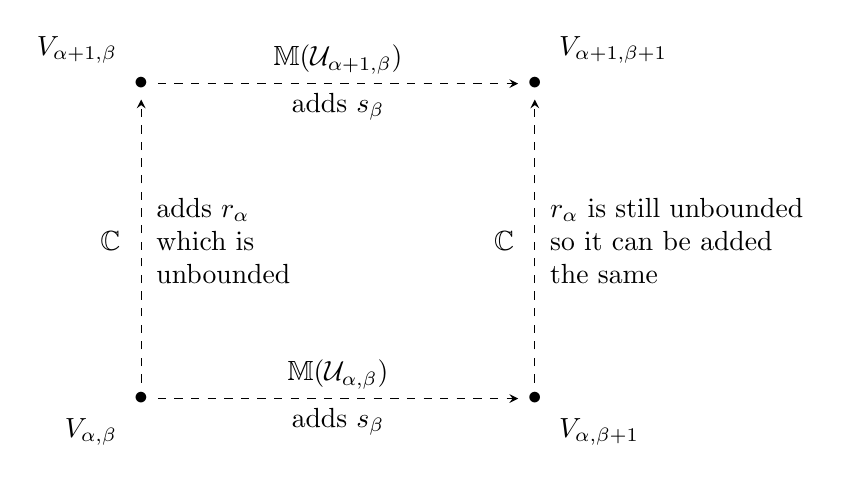
\begin{tikzpicture}[node distance=5cm, auto, >=stealth]
    % Define nodes with bullet dots and precise label distance
    \node[label={[label distance=-1pt]215:$V_{\alpha, \beta}$}] (Vab) at (0,0) {$\bullet$};
    \node[label={[label distance=-1pt]145:$V_{\alpha+1, \beta}$}] (Va1b) at (0,4) {$\bullet$};
    \node[label={[label distance=-1pt]325:$V_{\alpha, \beta+1}$}] (Vab1) at (5,0) {$\bullet$};
    \node[label={[label distance=-1pt]35:$V_{\alpha+1, \beta+1}$}] (Va1b1) at (5,4) {$\bullet$};

    % Bottom arrow: V_{\alpha, \beta} -> V_{\alpha, \beta+1}
    \draw[->, dashed] (Vab) -- (Vab1) 
      node[midway, above] {$\mathbb{M}(\mathcal{U}_{\alpha, \beta})$}
      node[midway, below] {adds $s_\beta$};

    % Top arrow: V_{\alpha+1, \beta} -> V_{\alpha+1, \beta+1}
    \draw[->, dashed] (Va1b) -- (Va1b1) 
      node[midway, above] {$\mathbb{M}(\mathcal{U}_{\alpha+1, \beta})$}
      node[midway, below] {adds $s_\beta$};

    % Left arrow: V_{\alpha, \beta} -> V_{\alpha+1, \beta}
    \draw[->, dashed] (Vab) -- (Va1b) 
      node[midway, left=4pt] {$\mathbb{C}$}
      node[midway, right=2pt, align=left] {adds $r_\alpha$ \\ which is \\ unbounded};

    % Right arrow: V_{\alpha, \beta+1} -> V_{\alpha+1, \beta+1}
    \draw[->, dashed] (Vab1) -- (Va1b1) 
      node[midway, left=4pt] {$\mathbb{C}$}
      node[midway, right=2pt, align=left] {$r_\alpha$ is still unbounded \\ so it can be added \\ the same};
  \end{tikzpicture}
\end{figure}

\newpage

\section*{Constructing the ultrafilters (formally)}

T.B.D.

\section*{Why $\domnumber = \continuum = \lambda$?}

T.B.D.

\newpage

\bibliographystyle{acm}
\bibliography{../refs.bib}
\end{document}
